\documentclass[xcolor=table, 10pt, aspectratio=1610]{beamer}

%\usepackage{arev}
\usepackage{amsmath,amssymb,amscd}
\usepackage{dsfont}
\usepackage{mathrsfs}
\usepackage{yfonts}
\usepackage{bm}
\usepackage{graphicx}
\usepackage{tabularx}
\usepackage{animate}
%\usepackage{mathtools}
%\usepackage{ifthen}

%\usepackage{xeCJK}
%\usepackage{fontspec}
%\newfontfamily\cjkfont{PingFang SC}
%\setCJKmainfont{PingFang SC}
\newcolumntype{x}{>{\centering\arraybackslash}X}
\renewcommand{\arraystretch}{1.5}
\newcommand{\uone}{\mathrm U(1)}
\DeclareMathOperator{\img}{img}

\usepackage{tikz}
	\usetikzlibrary{calc}
	\usetikzlibrary{arrows,shapes, positioning, matrix}
	\usetikzlibrary{decorations.markings}
	\tikzset{>=stealth}
	\tikzstyle arrowstyle=[scale=1]
	\tikzstyle directed=[postaction={decorate,decoration={markings,
 	   mark=at position .15 with {\arrow[arrowstyle]{stealth}}}}]
\tikzstyle string=[thick,postaction={decorate,decoration={markings,
    mark=at position .55 with {\arrow[arrowstyle]{stealth}}}}]
\tikzstyle dual_string=[dashed,postaction={decorate,decoration={markings,
    mark=at position .55 with {\arrow[arrowstyle]{stealth}}}}]

\tikzstyle dw=[thick,postaction={decorate,decoration={markings,
    mark=at position 1 with {\arrow[arrowstyle]{stealth}}}}]
\tikzstyle group=[mbg]
\newcommand*{\halfway}{0.5*\pgfdecoratedpathlength+.5*8pt}\tikzstyle arrowstyle=[scale=1]
\newcommand*{\halfwayb}{0.5*\pgfdecoratedpathlength}
\tikzstyle arrowstyle=[scale=1]
\tikzstyle fermion=[thick,postaction={decorate},decoration={markings,
    mark=at position \halfway with {\arrow[arrowstyle]{latex}}}]
\tikzstyle fermion2=[thick,postaction={decorate},decoration={markings,
        mark=at position \halfwayb with {\arrow[arrowstyle]{latex}}}]

\usepackage{pgffor}
\newcommand{\mb}[1]{\mathbf{#1}}
\renewcommand{\cal}[1]{\mathcal{#1}}

\newcommand{\ag}[2]{#1_\mb{#2}}
\newcommand{\cohosub}[1]{\scalebox{0.72}{\textswab{#1}}}
\newcommand{\cohosubsub}[1]{\scalebox{0.6}{\textswab{#1}}}
\newcommand{\coho}[1]{\textswab{#1}}

\DeclareMathOperator{\tr}{Tr}
\DeclareMathOperator{\im}{Im}
\DeclareMathOperator{\re}{Re}

\mode<presentation>
{
  %\usetheme{Warsaw}
  % or ...
  %\useoutertheme{rectangle}
  \setbeamertemplate{frametitle}[default][center]
  \defbeamertemplate{itemize item}{flat}{\begin{pgfpicture}{-1ex}{0ex}{1ex}{2ex}
      \pgfpathcircle{\pgfpoint{0pt}{.6ex}}{0.6ex}
      \pgfusepath{fill}
    \end{pgfpicture}%
  }
  \defbeamertemplate{itemize subitem}{flat}{\footnotesize\raise0.5pt\hbox{\textbullet}}
  \defbeamertemplate{itemize subsubitem}{flat}{\footnotesize\raise0.5pt\hbox{\textbullet}}

  %\useinnertheme{circles}
  \setbeamertemplate{items}[flat]
  \setbeamertemplate{sections/subsections in toc}[circle]
  \setbeamertemplate{blocks}[rounded]
  \setbeamertemplate{title page}[default][colsep=-4bp,rounded=true]
  \setbeamertemplate{part page}[default][colsep=-4bp,rounded=true]
  \setbeamercovered{transparent}
  %\usecolortheme{spruce}
  %\definecolor{THU}{RGB}{116,61,130}
  \definecolor{mbg}{RGB}{0,0,160}
  \setbeamercolor*{palette primary}{fg=white,bg=mbg}
  \setbeamercolor*{titlelike}{parent=palette primary}
  \setbeamercolor*{structure}{fg=mbg}
  \setbeamercolor{frametitle}{fg=white,bg=mbg}
  % or whatever (possibly just delete it)
  \setbeamercolor{block title}{bg=mbg,fg=white}
  \setbeamercolor{block body}{bg=mbg!15}


  \addtobeamertemplate{navigation symbols}{}{ \hspace{1em}%
    \usebeamerfont{footline}%
    \insertframenumber / \inserttotalframenumber }
}


%\usepackage[english]{babel}
% or whatever

%\usepackage[latin1]{inputenc}
% or whatever

%\usepackage{times}
%\usepackage[T1]{fontenc}
% Or whatever. Note that the encoding and the font should match. If T1
% does not look nice, try deleting the line with the fontenc.

\title[Space-group SPTs] % (optional, use only with long paper titles)
{Real-Space Recipes for General Topological Crystalline States}

\author[Y Qi] % (optional, use only with lots of authors)
{Yang~Qi}
% - Give the names in the same order as the appear in the paper.
% - Use the \inst{?} command only if the authors have different
%   affiliation.

\institute[Fudan] % (optional, but mostly needed)
{Department of Physics, Fudan University}
% - Use the \inst command only if there are several affiliations.
% - Keep it simple, no one is interested in your street address.

%\date{2016 Annual Meeting of Fudan CFTPP} % (optional, should be abbreviation of conference name)
%{Fudan University, Oct 13 2015}
\date{SUSTC, Dec. 2018}
% - Either use conference name or its abbreviation.
% - Not really informative to the audience, more for people (including
%   yourself) who are reading the slides online

\subject{Theoretical Physics}
% This is only inserted into the PDF information catalog. Can be left
% out.



% If you have a file called "university-logo-filename.xxx", where xxx
% is a graphic format that can be processed by latex or pdflatex,
% resp., then you can add a logo as follows:

\pgfdeclareimage[height=1cm]{university-logo}{../resources/fudan}
\logo{\pgfuseimage{university-logo}}


% Delete this, if you do not want the table of contents to pop up at
% the beginning of each subsection:

\begin{document}

\begin{frame}
  \titlepage
\end{frame}

\begin{frame}{References}
\begin{itemize}
\item Zhi-Da Song: Princeton University.
\item Chen Fang: Institute of Physics, Beijing.
\begin{center}
	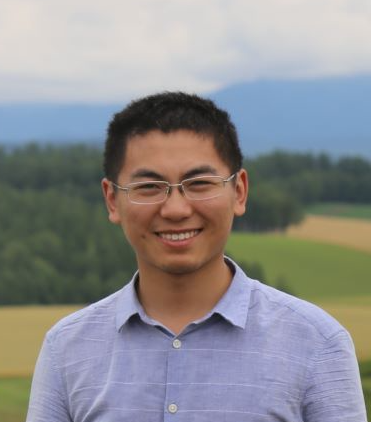
\includegraphics[height=3cm]{../people/zhidasong}
	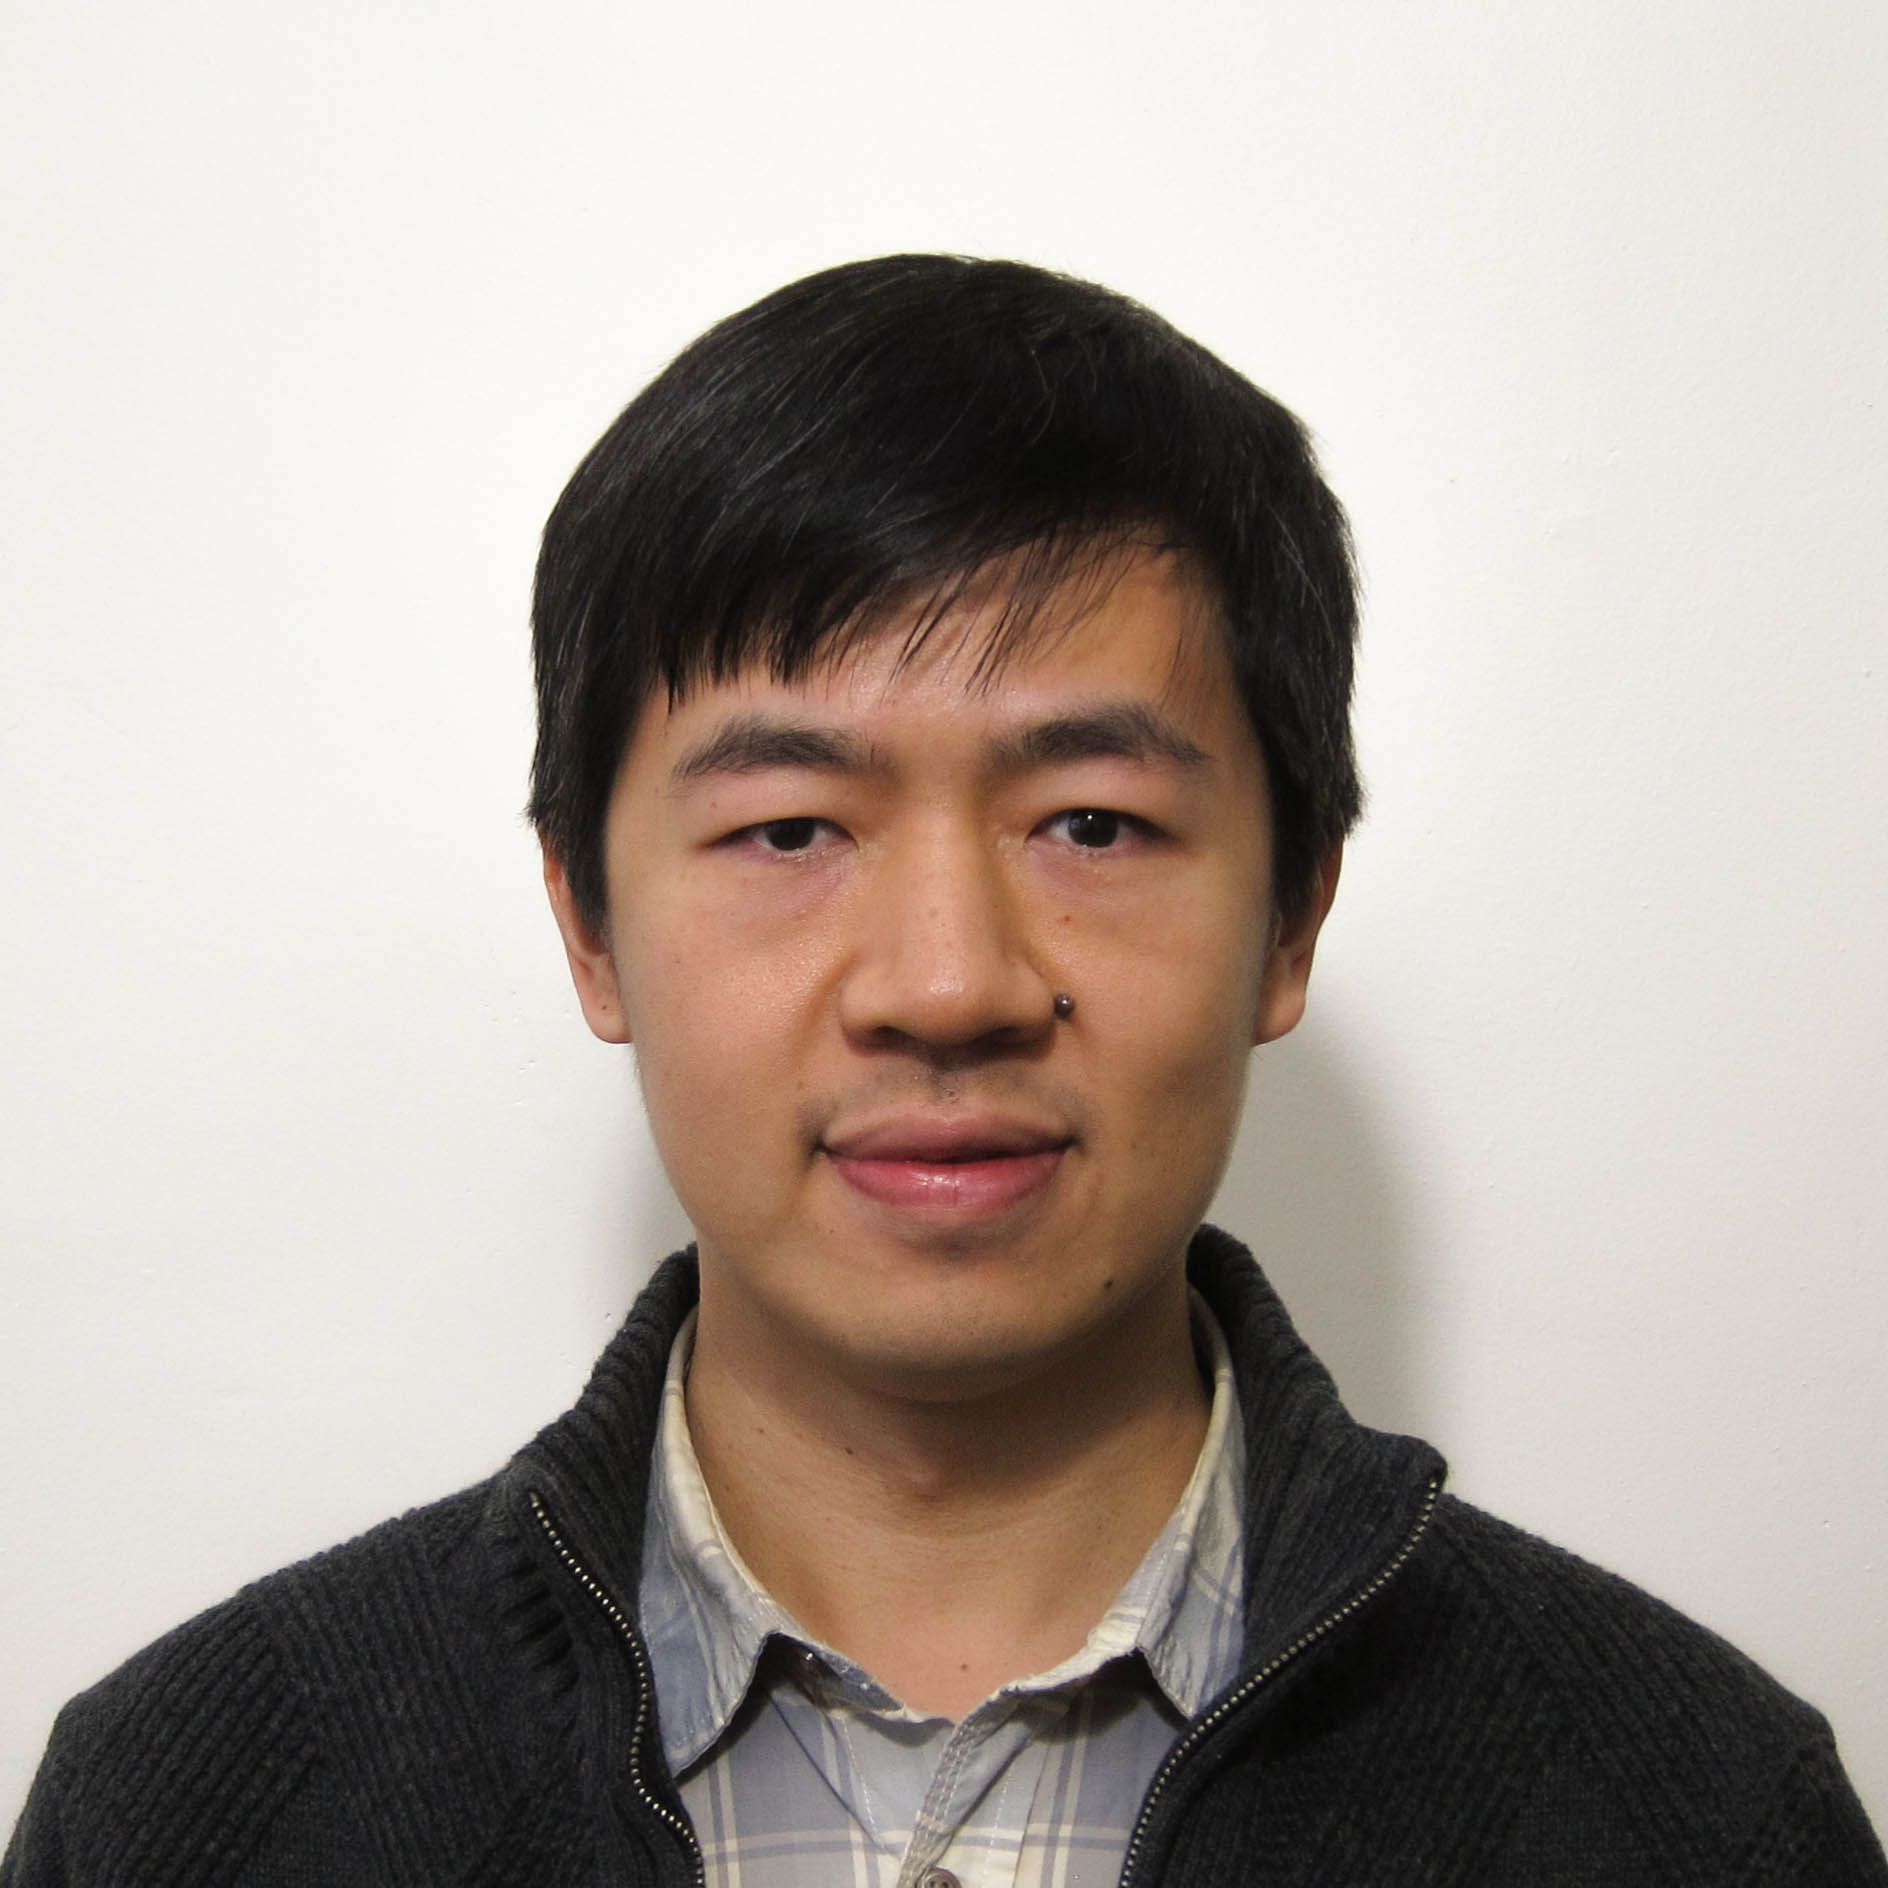
\includegraphics[height=3cm]{../people/chenfang}
\end{center}
\item Zhida Song, Chen Fang and Yang Qi, arXiv:1810.11013
\end{itemize}
\end{frame}

\section{Introduction to Symmetry-Protected Topological (SPT) states}

\begin{frame}
  \frametitle{Symmetry-Protected Topological (SPT) states}
\begin{itemize}
\item SPT: gapped topological phases beyond Landau paradiam.
\item Cannot be smoothly connected to a trivial state without closing gap or breaking symmetry.
\item Symmetry-protected gapless surface states.
\item Free-fermion states: topological insulators, topological superconductors.
\item Bosonic SPTs: Haldane chain, CZX/Levin-Gu state, etc.\\
\emph{Xie Chen, Zheng-Cheng Gu, Zheng-Xin Liu and Xiao-Gang Wen, Science 2012.}
\item Interacting fermionic SPTs.
\end{itemize}
\end{frame}

\begin{frame}
\frametitle{Space-group SPT}
\begin{itemize}
\item We consider $G/G_0 = SG$.
\item Thorngren and Else (2018): equivalence principle.
\[H^{d+1}[G, \uone_{PT}].\]
\item Dimensional reduction: Liang Fu, Michael Hermele et al.\\
\emph{Examples: mirror SPT, weak SPT (translation symmetry).}
\item A more general construction for SPTs w/ all possible $G$.
\end{itemize}
\begin{center}
\begin{tikzpicture}
\fill [blue!20] (0,0)--(1,1)--(1,3)--(0,2)--(0,0);
\draw (0,0)--(0,2)--(1,3);
\draw (-1.5,0)--(1.5,0)--(1.5,2)--(-1.5,2)--(-1.5,0);
\draw (1.5,0)--(2.5,1)--(2.5,3)--(1.5,2);
\draw (2.5,3)--(-.5,3)--(-1.5,2);
\end{tikzpicture}
\hspace{2em}
\begin{tikzpicture}
\fill [blue!40,opacity=.5] (0,0)--(1,1)--(1,3)--(0,2)--(0,0);
\draw (0,0)--(0,2)--(1,3);
\fill [blue!40,opacity=.5] (.5,0)--(1.5,1)--(1.5,3)--(0.5,2)--(0.5,0);
\draw (.5,0)--(.5,2)--(1.5,3);
\fill [blue!40,opacity=.5] (1,0)--(2,1)--(2,3)--(1,2)--(1,0);
\draw (1,0)--(1,2)--(2,3);
\fill [blue!40,opacity=.5] (-.5,0)--(.5,1)--(.5,3)--(-0.5,2)--(-0.5,0);
\draw (-.5,0)--(-.5,2)--(.5,3);
\fill [blue!40,opacity=.5] (-1,0)--(0,1)--(0,3)--(-1,2)--(-1,0);
\draw (-1,0)--(-1,2)--(0,3);
\draw (-1.5,0)--(1.5,0)--(1.5,2)--(-1.5,2)--(-1.5,0);
\draw (1.5,0)--(2.5,1)--(2.5,3)--(1.5,2);
\draw (2.5,3)--(-.5,3)--(-1.5,2);
\end{tikzpicture}
\end{center}
\end{frame}

\section{Simplified version: 1st and 2nd pages.}
\begin{frame}
	\frametitle{Topological crystalline states are made of building blocks}
	\begin{columns}
		\column{.4\textwidth}
		\begin{center}
			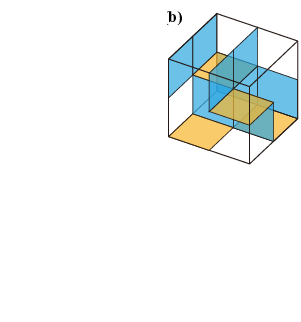
\includegraphics[width=\textwidth]{blocks}
		\end{center}
		\column{.6\textwidth}
		\begin{itemize}
			\item We divide the space into cells compatible with the space-group symmetry.
			\item On a $p$-cell $\sigma$, the SPT state is protected only by $G_\sigma$.
			\[\hat\omega(\sigma)\in \Phi^d(G).\]
			\item $G_\sigma$ acts as onsite symmetries.
			\item Decorate 3d SPT on 3-cells; 2d SPT on 2-cells; 1d SPT on 1-cells; 0d SPT on 0-cells;
			\item $p$-block states: $E^p_{p,\infty}$.
			\[\text{TCSs} = \bigoplus_p E^p_{p,\infty}.\]
		\end{itemize}
	\end{columns}
\end{frame}

\begin{frame}
	\frametitle{Decomposition of the space}
	We divide the space into finer cells such that
	\begin{enumerate}
		\item A cell $\sigma$ is maped to one single cell $\sigma^\prime$ under $SG$-action.
		\item $G_\sigma$ acts on $\sigma$ as onsite symmetry.
	\end{enumerate}
	\begin{center}
		\begin{tikzpicture}
			\draw (-2, -2)--(-2, 2)--(2, 2)--(2, -2)--(-2, -2);
			\draw [thick] (0, -2)--(0, 2);
			\filldraw (0, 0) circle (1pt) node [right] {$C_2$};
			\node at (0, -1) [right] {$\tau_1$};
			\node at (0, 1) [left] {$\tau_2$};
			\node at (-1, 0) {$\sigma_1$};
			\node at (1, 0) {$\sigma_2$};
		\end{tikzpicture}
	\end{center}
\end{frame}

\begin{frame}
	\frametitle{Symmetric conditions}
	\begin{columns}
		\column{.4\textwidth}
		\begin{tikzpicture}
			\draw (0, 0)--(2, 0)--(2, 2)--(0, 2)--(0, 0);
			\draw (2, 4)--(4, 4)--(4, 6)--(2, 6)--(2, 4);
			\draw [thick,->] (1, 1) node [below] {$\hat\omega(\sigma$)} --
			(3, 5) node [above] {$\hat\omega(\sigma^\prime)$};
			\node at (2, 3) [right] {$g$};
		\end{tikzpicture}
		\column{.6\textwidth}
		\begin{itemize}
			\item If $g:\sigma\rightarrow\sigma^\prime$, then the cochains attached must be ``identical''.
			\item $G_\sigma\neq G_{\sigma'}$, but they are isomorphic:
			\[G_{\sigma'}=gG_\sigma g^{-1}\simeq G_\sigma.\]
			\item This induces another isomorphism between the cohomology classes:
			\[H^{p+1}[G_{\sigma'},\uone_T]\simeq H^{p+1}[G_\sigma,\uone_T]\]
			\item $\hat\omega(\sigma)$ and $\hat\omega(\sigma')$ are related by this isomorphism, which we denote by
			\[\hat\omega(\sigma') = g\cdot \hat\omega(\sigma).\]
			\item Only decorations on symmetry-unrelated cells are independent: finite \# of them.
		\end{itemize}
	\end{columns}
\end{frame}

\begin{frame}
	\frametitle{The 1st page}

	\begin{columns}
		\column{.4\textwidth}
		\begin{center}
			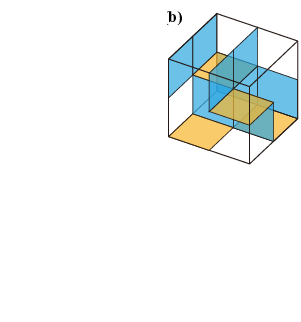
\includegraphics[width=\textwidth]{blocks}
		\end{center}
		\column{.6\textwidth}
		\begin{itemize}
			\item 1st page = a collection of SPTs:
			\[E^p_{p,1} = \bigoplus_{\sigma\in Y_p/G} \Phi^p(G_\sigma),\]
			\[\Phi^p(G_\sigma) = H^{p+1}(G_\sigma, \uone_T).\]
			\item We can generalize this to
			\[E^q_{p,1} = \bigoplus_{\sigma\in Y_p/G} \Phi^q(G_\sigma).\]
		\end{itemize}
	\end{columns}
\end{frame}

\begin{frame}
	\frametitle{No-Open-Edge Conditions}
	\begin{columns}
		\column{.58\textwidth}
		\begin{itemize}
			\item SPT blocks have nontrivial boundary states.
			\item Boundary anomaly must cancel on $(p-1)$-cells.
			\item Naively:
			\[\hat\omega(\sigma_1)
			+\hat\omega(\sigma_2)+\hat\omega(\sigma_3)+\hat\omega(\sigma_4)\]
			\item A subtlety: $\tau$ has more symmetry operations than $\sigma$: $G_\tau \supseteq G_\sigma$
			\item Hence, $\hat\omega(\sigma_i)$ is not $G_\tau$-symmetric.
			\item When $[G_\tau:G_\sigma]>1$: $\tau$ borders $[G_\tau:G_\sigma]$ symmetry-related copies of $\sigma_i$.
			\item $\hat\omega(\sigma_1)
			+\hat\omega(\sigma_2)+\hat\omega(\sigma_3)+\hat\omega(\sigma_4)\in H^{p+1}[G_\tau,\uone_T]$.
		\end{itemize}
		\column{.42\textwidth}
		\begin{tikzpicture}
			\draw (0, 1)--(-1, 1)--(-2, 0)--(2, 0)--(3, 1)--(1, 1);
			\draw [thick] (0, 0)--(1, 1);
			\node at (.5, .5) [above] {$\tau$};
			\draw (1, 1)--(1, 3)--(0, 2)--(0, -2)--(0, -2)--(1, -1)--(1, 0);
			\node at (.5, 1.5) {$\sigma_1$};
			\node at (1.5, .5) {$\sigma_2$};
			\node at (.5, -0.5) {$\sigma_3$};
			\node at (-0.5, .5) {$\sigma_4$};
		\end{tikzpicture}
	\end{columns}
\end{frame}

\begin{frame}
	\frametitle{No-Open-Edge Conditions}
	\begin{columns}
		\column{.58\textwidth}
		\begin{itemize}
			\item We can define a boundary-transfer operation $\partial\omega$:
			\[(\partial\omega)(\tau)=\hat\omega(\sigma_1)
			+\hat\omega(\sigma_2)+\hat\omega(\sigma_3)+\hat\omega(\sigma_4).\]
			\item Cocycle equation: $\partial\omega\simeq0.$
			\item Define $d_1: E^p_{p,1}\rightarrow E^p_{p-1,1}$:
			\[d_1\omega = \partial\omega.\]
			\item First-page no-open-edge condition:
			\[d_1\omega \simeq 0.\]
			\item $E^{p+1}_{p,r}$: anomaly pattern.
		\end{itemize}
		\column{.42\textwidth}
		\begin{tikzpicture}
			\draw (0, 1)--(-1, 1)--(-2, 0)--(2, 0)--(3, 1)--(1, 1);
			\draw [thick] (0, 0)--(1, 1);
			\node at (.5, .5) [above] {$\tau$};
			\draw (1, 1)--(1, 3)--(0, 2)--(0, -2)--(0, -2)--(1, -1)--(1, 0);
			\node at (.5, 1.5) {$\sigma_1$};
			\node at (1.5, .5) {$\sigma_2$};
			\node at (.5, -0.5) {$\sigma_3$};
			\node at (-0.5, .5) {$\sigma_4$};
		\end{tikzpicture}
	\end{columns}
\end{frame}

\begin{frame}
	\frametitle{Bubbling Equivalence}
\begin{columns}
\column{.6\textwidth}
\begin{itemize}
\item Coboundaries: $\omega\simeq0$.
\item A coboundary: attaching the same SPT state to  $\partial \sigma$.
\item The bubbling process can also expressed by $\partial$:
\[\omega = \partial\mu\simeq0.\]
\item We define $d_1:E^p_{p+1, 1}\rightarrow E^p_{p,1}$:
\[d_1\mu = \partial\mu.\]
\item The first-page bubbling equivalence:
\[d_1\mu\simeq0.\]
\item $E^{p+1}_{p,r}$: Bubbling patterns.
\end{itemize}
\column{.4\textwidth}
\begin{animateinline}{5}
        \multiframe{12}{Ra=.8+.1}{
\begin{tikzpicture}
	\draw (-2,-2)--(-2,2)--(2,2)--(2,-2)--(-2,-2);
	%\fill [green!30] (-\Ra,-\Ra)--(-\Ra,\Ra)--(\Ra,\Ra)--(\Ra,-\Ra)--(-\Ra,-\Ra);
\draw [blue,thick] (-\Ra,-\Ra)--(-\Ra,\Ra)--(\Ra,\Ra)--(\Ra,-\Ra)--(-\Ra,-\Ra);
%\node at (0, 0) {$d\nu$};
\node at (\Ra, 0) [left] {$\nu$};
\end{tikzpicture}
}
\end{animateinline}
\end{columns}
\end{frame}

\begin{frame}
\frametitle{2nd page: a homology-group calculation}
\begin{itemize}
\item No-open-edge conditions:
\[d_1\omega\simeq 0.\]
\item Bubbling equivalence:
\[d_1\mu\simeq 0.\]
\item A homology-group calculation:
\[E^p_{p+1,1}\xrightarrow{d_1}E^p_{p,1}\xrightarrow{d_1}E^p_{p-1,1},\]
\[E^p_{p,2}=\frac{\ker d^p_{p+1,1}}{\img d^p_{p,1}}.\]
\end{itemize}
\end{frame}

\begin{frame}
	\frametitle{Free-fermion decoration}
	\begin{columns}
		\column{.4\textwidth}
		\begin{center}
			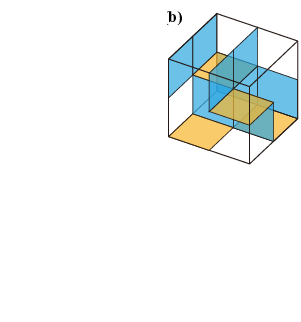
\includegraphics[width=\textwidth]{blocks}
		\end{center}
		\column{.6\textwidth}
		\begin{itemize}
			\item Time-reversal + charge U(1): AII class
			\item Generic 2D plane: decorate 2D TI, $\mathbb Z_2$ classification.
			\[H_2(\mathbb R^3 / SG, \mathbb Z_2).\]
			\item Mirror 2D plane: decorate mirror TCI, $\mathbb Z$ classification.
			\item Zhida Song, Sheng-Jie Huang, Yang Qi, Chen Fang, Michael Hermele, arXiv:1810.02330
		\end{itemize}
	\end{columns}
\end{frame}

\begin{frame}
	\frametitle{Free-fermion decoration}
	\begin{columns}
		\column{.4\textwidth}
		\begin{center}
			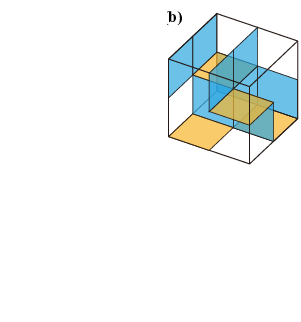
\includegraphics[width=\textwidth]{blocks}
		\end{center}
		\column{.6\textwidth}
		\begin{itemize}
			\item Charge U(1): AI class
			\item Generic 2D plane: decorate Chern insulators, $\mathbb Z$ classification.
			\[H_2(\mathbb R^3 / SG, \mathbb Z).\]
			\item Mirror 2D plane: decorate mirror TCI, $\mathbb Z$ classification.
			\item Work in progress.
		\end{itemize}
	\end{columns}
\end{frame}

\begin{frame}
	\frametitle{Bosonic SPT (group cohomology) decoration}
	\begin{columns}
		\column{.4\textwidth}
		\begin{center}
			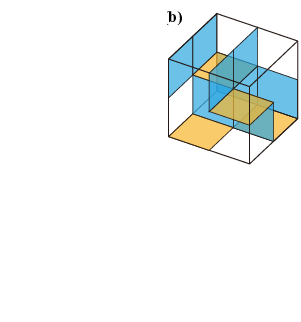
\includegraphics[width=\textwidth]{blocks}
		\end{center}
		\column{.6\textwidth}
		\begin{itemize}
			\item Arbitrary symmetry group $G/G_0=SG$.
			\item Decorate 3d SPT on 3-cells; 2d SPT on 2-cells; 1d SPT on 1-cells; 0d SPT on 0-cells.
			\item $\Phi^d(G_\sigma) = H^{d+1}[G_\sigma, \uone_T]$.
			\item Spectral sequence:
			\[E^p_{p, 1}=\sum_{\sigma\in Y_p}H^{p+1}[G_\sigma, \uone_T]
			\Rightarrow H^{d+1}[G, \uone_{PT}].\]
			\item Zhida Song, Chen Fang and YQ, arXiv:1810.11013
			\item D. Else and R. Thorngren, arXiv:1810.10539
		\end{itemize}
	\end{columns}
\end{frame}

\begin{frame}
	\frametitle{Interacting-fermion SPT (group cohomology) decoration}
	\begin{columns}
		\column{.4\textwidth}
		\begin{center}
			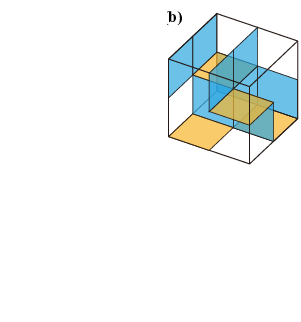
\includegraphics[width=\textwidth]{blocks}
		\end{center}
		\column{.6\textwidth}
		\begin{itemize}
			\item Arbitrary symmetry group $G/G_0=SG$.
			\item Decorate 3d SPT on 3-cells; 2d SPT on 2-cells; 1d SPT on 1-cells; 0d SPT on 0-cells.
			\item $\Phi^d(G_\sigma) = ??$.
		\end{itemize}
	\end{columns}
\end{frame}

\begin{frame}
	\frametitle{SET decoration}
	\begin{columns}
		\column{.3\textwidth}
		\begin{center}
		\begin{tikzpicture}
		\draw (-1.2,0)--(1.2,0);
		\draw (-1.2,1)--(1.2,1);
		\draw (-1.2,-1)--(1.2,-1);
		\draw (-1,-1.2)--(-1,1.2);
		\draw (0,-1.2)--(0,1.2);
		\draw (1,-1.2)--(1,1.2);
		\fill [red] (-1,-1) circle (2pt);
		\fill [red] (-1,0) circle (2pt);
		\fill [red] (-1,1) circle (2pt);
		\fill [red] (0,-1) circle (2pt);
		\fill [red] (0,0) circle (2pt);
		\fill [red] (0,1) circle (2pt);
		\fill [red] (1,-1) circle (2pt);
		\fill [red] (1,0) circle (2pt);
		\fill [red] (1,1) circle (2pt);
		\end{tikzpicture}
		\end{center}

		\column{.7\textwidth}
		\begin{itemize}
			\item 2-cells: intrinsic topological order w/o symmetry.
			\item 1-cells: gluing together w.r.t. $G_\sigma=\mathbb Z_2$ mirror symmetry.\\
			YQ, Chao-Ming Jian and Chenjie Wang, arXiv:1710.09391
			\item 0-cells: gluing together 1D boundaries?
		\end{itemize}
\end{columns}

\end{frame}

\begin{frame}
	\frametitle{A computational program}
	\begin{itemize}
		\item Constructing a CW-complex compatible with a $SG$: Zhida Song.
		\item Computing group cohomology: GAP (www.gap-system.org).
		\item Computing homology groups / spectral sequences.
		\item Cohomology operations: cup product, higher-cup product, ... ?
	\end{itemize}
\end{frame}
%\begin{frame}
%	\frametitle{A building block}
%	\begin{columns}
%		\column{.4\textwidth}
%		\begin{center}
%			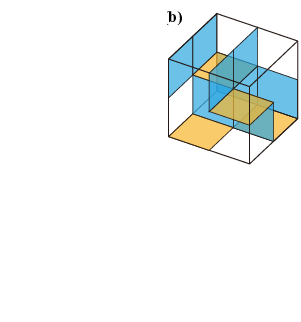
\includegraphics[width=\textwidth]{blocks}
%		\end{center}
%		\column{.6\textwidth}
%		\begin{itemize}
%			\item A building block $\hat\omega$ is a collection of cochains:
%			\[\hat\omega(\sigma) \in C^{p+1}[G_\sigma, \uone_T].\]
%			\item $\hat\omega$ needs to be symmetric under $SG$.
%			\item $\hat\omega$ needs to satisfy the bulk-boundary relation:
%			\[d\hat\omega(\tau) = \sum_{\sigma:\tau\in\partial\sigma}\hat\omega(\sigma).\]
%			\item Need to find when two blocks can be deformed to each other: $\hat\omega\simeq\hat\omega^\prime$.
%		\end{itemize}
%	\end{columns}
%\end{frame}



\end{document}
